\chapter{Dynamical Processes in Biomedicine}
\label{cha:bio_background}

\dictum[Rosalind Franklin, \textit{Report} (1952)]{%
  The results suggest a helical structure (which must be very closely packed) containing probably 2, 3 or 4 coaxial nucleic acid chains per helical unit and having the phosphate groups near the outside.}%
\vskip 1em

...


\chapter{Optimal Transport for Dynamical Systems}
\label{cha:theory_background}

\dictum[Elinor Ostrom, \textit{Governing the Commons} (1990)]{%
  The power of a theory is exactly proportional to the diversity of situations it can explain.}%
\vskip 1em


Optimal transport theory~\citep{santambrogio2015optimal} is a core element of the machine learning toolbox and has become within a few years the go-to framework to analyze, model, and solve an ever-increasing variety of tasks involving probability measures. This is best exemplified by its increasing importance to fitting generative models, where the goal is to learn a map~\citep{arjovsky2017wasserstein, genevay2018learning, salimans2018improving}, or more generally a diffusion \citep{song2020score, de2021diffusion} to morph a simple measure (e.g., Gaussian) onto a data distribution of interest (e.g., images). This is also apparent in the many applications that use OT to align probability measures that have since arisen, e.g., to transfer label knowledge between datasets~\citep{flamary2016optimal, singh2020model}, to analyze sampling schemes~\citep{dalalyan2017theoretical}, or study population trajectories~\citep{schiebinger2019optimal, bunne2021learning}.

In this chapter, we primarily cast light on the static and dynamic formulation of optimal transport, and simultaneously establish their theoretical nexus by recalling its mathematical history from \citet{monge1781histoire} and \citet{kantorovich1942transfer} to modern Fields Medal winners \citet{villani2009optimal}, \citeauthor{figalli2010optimal}, and Abel Prize recipient \citet{caffarelli1990interior} in order to provide a solid foundation for the discussion ahead.


\section{Static Optimal Transport} \label{sec:background_ot_static}

\looseness -1 Optimal transport takes dual roles as it induces a mathematically well-characterized distance measure between distributions as well as provides a geometry-based approach to realize mappings between two probability distributions.
In this section, we introduce the mathematical foundations of the \textbf{static} OT problem. Further, we will provide an extended analysis of the \citeauthor{monge1781histoire} map, which provides an actionable way to flow from one probability distribution onto another.
We conclude with a complete proof of the celebrated \citeauthor{brenier1987decomposition} theorem. This quintessential result and its particularization to translation-invariant costs will lay the foundation of the flurry of neural approaches proposed in the literature. This includes modeling Monge maps as gradients of convex functions parameterized through convex neural networks \citep{amos2017input, huang2021convex, makkuva2020optimal, korotin2021neural, lubeck2022neural, bunne2022supervised}, i.e., approaches that are a direct consequence of the \citeauthor{brenier1987decomposition} theorem and subject of this thesis, regularizers \citep{uscidda2023monge}, amortized optimization \citep{amos2022amortizing, amos2022meta}, or entropic maps \citep{pooladian2021entropic, pooladian2023minimax, divol2022optimal, cuturi2023monge}.

\begin{figure}[t]
  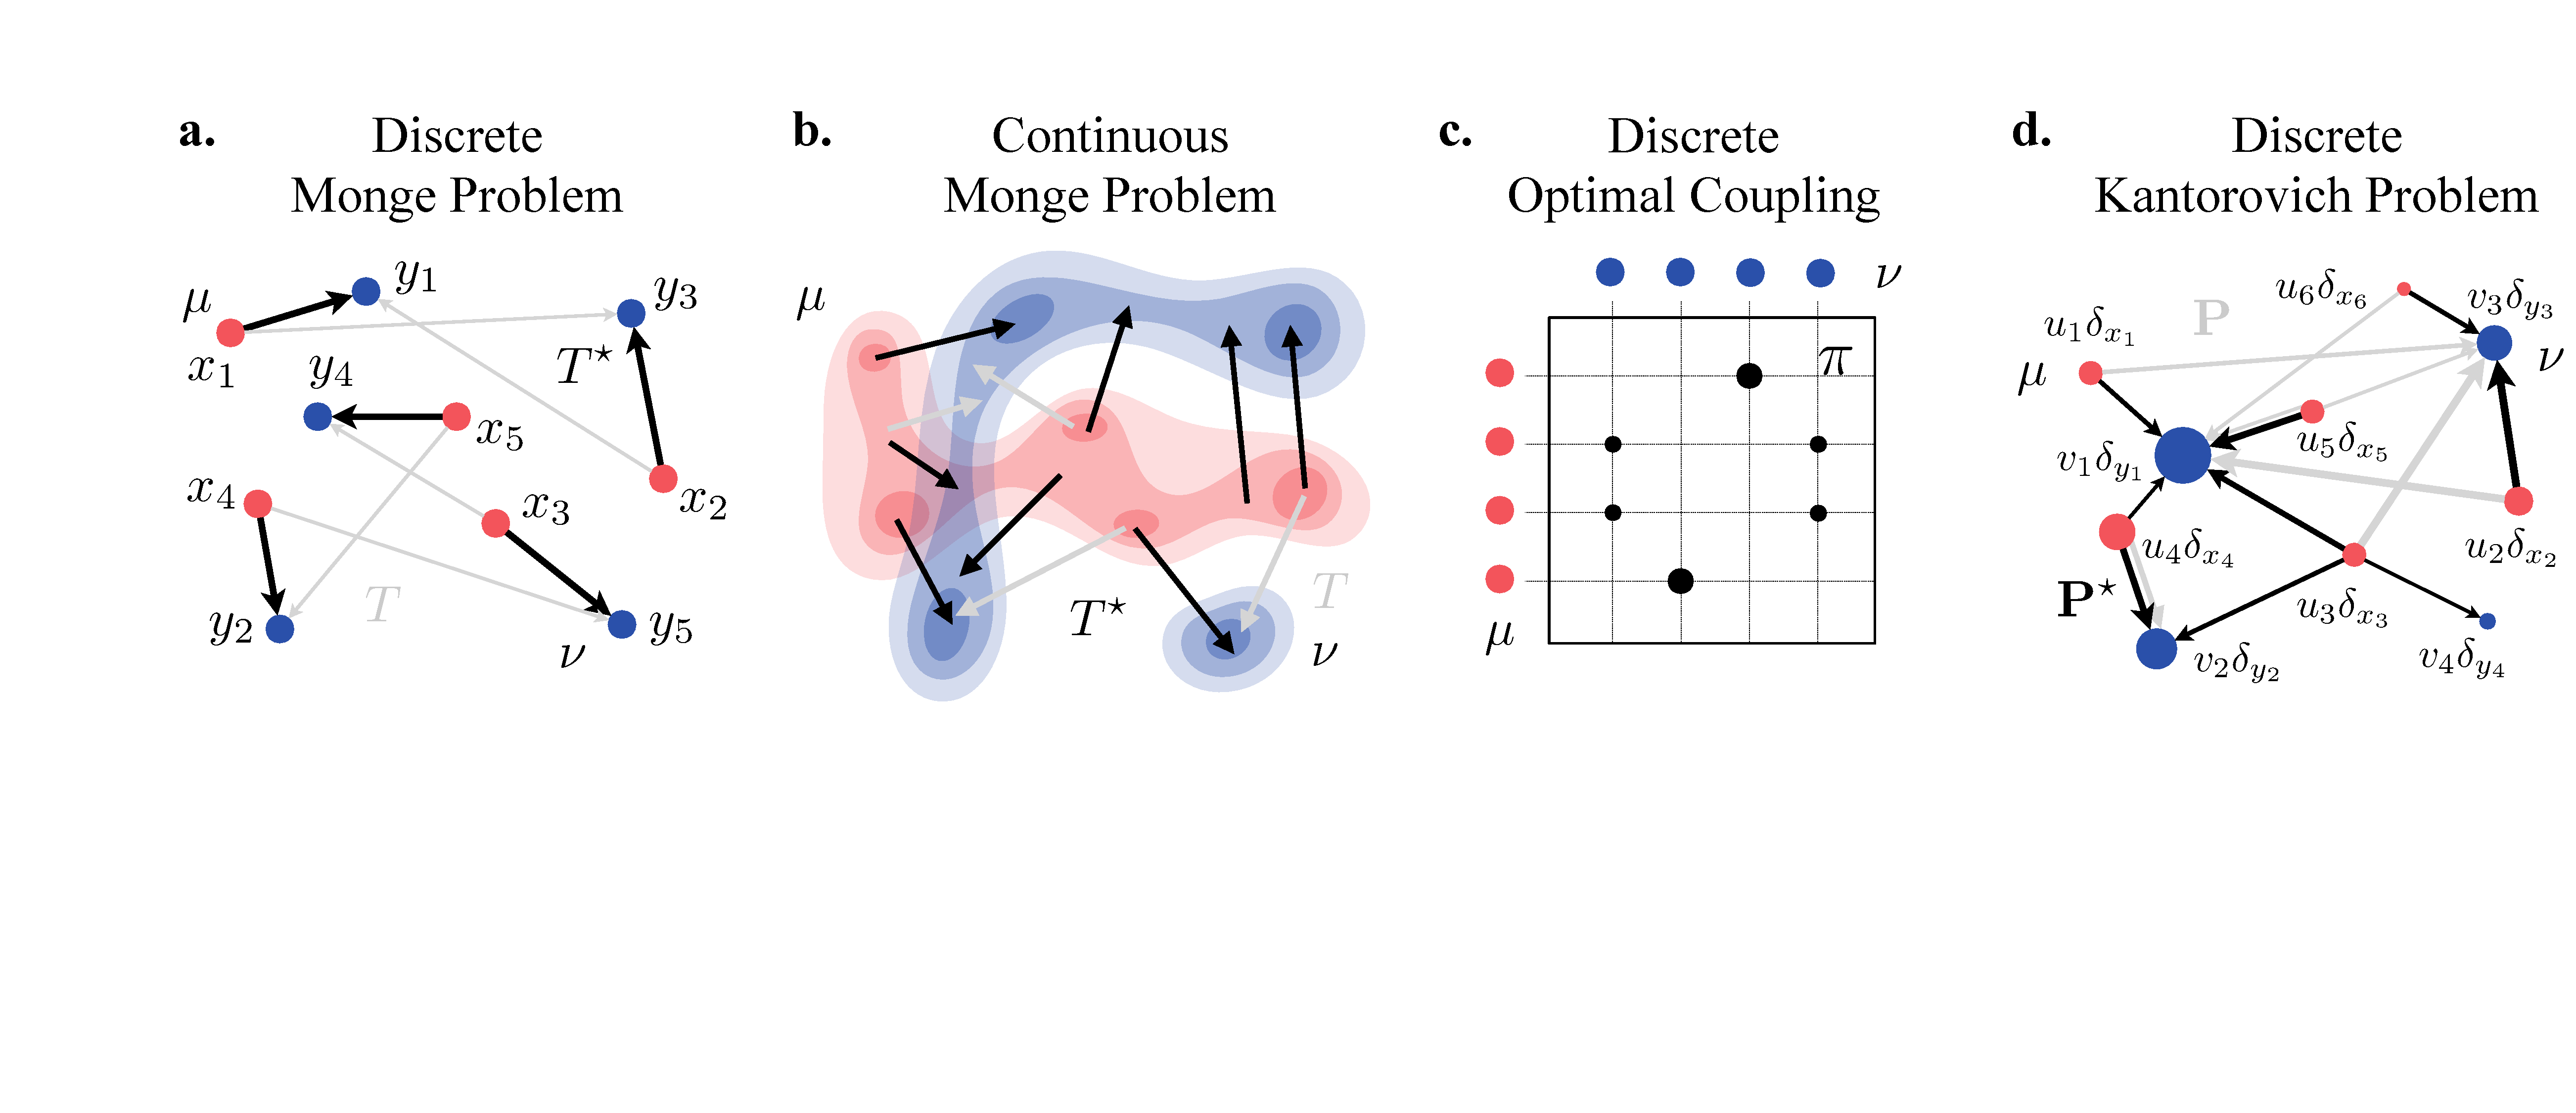
\includegraphics[width=\textwidth]{figures/fig_ot_background.pdf}
  \caption{\textbf{Overview on different formulations of the static OT problem for discrete and continuous measures.} Monge map for \textbf{a.} discrete and\textbf{b.} continuous measures $\mu, \nu$. The optimal map $T^\star$ minimizes \eqref{eq:monge}. \textbf{c.} Optimal coupling $\pi$ \eqref{eq:kantorovich} for discrete measures $\mu$ and $\nu$. \textbf{d.} Mass splitting principle of the Kantorovich relaxation for discrete measures $\mu$ and $\nu$ of the optimal transport plan $\bP^\star$ and a non-optimal plan $\bP$. Figure adapted from \citet{peyre2019computational}.}	
  \label{fig:ot_principles}
\end{figure}

\subsection{Monge Problem} \label{sec:background_monge}

In the 18th century "M{\'e}moire sur la th{\'e}orie des d{\'e}blais et des remblais", Gaspard Monge sets out to solve what is now known as the \citeauthor{monge1781histoire} problem, posing a seemingly simple, yet fundamentally complex question: Given two quantities of mass located at two different sites, what is the most efficient way into transport one to the other?
In more formal terms, provided with two measures $\mu, \nu\in \mathcal{P}(\mathbb{R}^d)$, here restricted to measures supported on $\mathbb{R}^d$, Monge's initial approach was to find a map $T$ that pushes one mass onto the other in a way that minimizes the total cost of transport.
Given a measurable const function $c: \mathcal{X} \times \mathcal{Y} \rightarrow \mathbb{R}$, the \citeauthor{monge1781histoire} problem then reads
\begin{equation}\label{eq:monge}
T^\star := \arg\inf_{T\sharp\mu=\nu}\int_{\mathbb{R}^d} c(x, T(x)) d\mu(x)\,.
\end{equation}
For two discrete measures $\mu=\sum_{i=1}^n u_i \delta_{x_{i}}, \nu=\sum_{j=1}^m v_j \delta_{y_{j}}$, it seeks a transport map $T: \mathcal{X} \rightarrow \mathcal{Y}$ associating each source point $x_i$ to a target point $x_j$ (see \cref{fig:ot_principles}a for the discrete and \cref{fig:ot_principles}b for the continuous setting).
...
The existence of $T^\star$ is guaranteed under fairly general conditions \citep[Theorem 1.22]{santambrogio2015optimal}, which require that $\mu$ and $\nu$ have finite $L_2$ norm, and that $\mu$ puts no mass on $(d-1)$ surfaces of class $\mathcal{C}_2$.


\subsection{Kantorovich Relaxation} \label{sec:background_kantorovich}

It was not until the 20th century, however, that the concept found a more tractable development. In \citeyear{kantorovich1942transfer}, Leonid \citeauthor{kantorovich1942transfer} provided a relaxation to this non-convex and difficult-to-solve problem.
Instead of the deterministic matching proposed by \citeauthor{monge1781histoire}, Kantorovich considered probabilistic correspondences that allow for transportation of mass from a single source point to various target points (mass splitting), resulting in
\begin{equation} \label{eq:kantorovich}
    W(\mu, \nu) = \inf_{\pi\in \Pi(\mu,\nu)}\iint c(x, y) \pi(dx, dy),
\end{equation}
where $\Pi(\mu, \nu) \defeq \left\{\pi \in \gP(\mathcal{X} \times \mathcal{Y}): P_{\gX \sharp} \pi=\mu \, \text { and } \, P_{\gY \sharp} \pi=\nu\right\}$ is the set of couplings on $\mathbb{R}^d\times\mathbb{R}^d$ with respective marginals $\mu, \nu$ (see \cref{fig:ot_principles}c).
For his work, \citeauthor{kantorovich1942transfer} received the Nobel Prize in economics. The connections of \acrshort{OT} to basic questions in economy becomes clear when interpreting $\mu$ as a density of resource units, and $\nu$ a density of factories, where the coupling $\pi$ denotes the optimal transportation plan of distributing resources to factories.

When instantiated on finite discrete measures, such as $\mu=\sum_{i=1}^n u_i\delta_{x_i}$ and $\nu=\sum_{j=1}^m v_j\delta_{y_j}$, this problem translates to a linear program, which can be regularized using an entropy term~\citep{cuturi2013sinkhorn,peyre2019computational}. For $\varepsilon\geq0$, set 
\begin{equation} \label{eq:reg-ot}
\We(\mu,\nu) \defeq \min_{\bP\in U(u, v)} \dotp{\bP}{[c(x_i, y_j)]_{ij}}  \,-\varepsilon H(\bP),
\end{equation}
where the discrete entropy is defined as $H(\bP) \defeq -\sum_{ij} \bP_{ij} (\log \bP_{ij} - 1)$ and the polytope $U(u, v)$ is the set of $n\times m$ matrices $\{\bP\in\mathbb{R}^{n \times m}_+, \bP\mathbf{1}_m =u, \bP^\top\mathbf{1}_n=v\}$. 
Notice that the definition above reduces to the usual Wasserstein distance when $\varepsilon=0$. Setting $\varepsilon>0$ yields a faster and differentiable proxy to approximate $W_{0}$, but introduces a bias, since $\We(\mu,\mu)\ne 0$ in general.
Thus, regularizing objective \eqref{eq:kantorovich} with an entropy term results in a significantly more efficient optimization \citep{cuturi2013sinkhorn} and differentiability w.r.t. its inputs. As a consequence, \eqref{eq:reg-ot} is commonly used as a loss function in machine learning applications, e.g., for structured prediction \citep{frogner2015learning,janati2020multi} or generative model fitting \citep{arjovsky2017wasserstein, salimans2018improving, genevay2018learning}.


\subsection{Kantorovich Duality} \label{sec:background_dual}

The Kantorovich formulation \eqref{eq:kantorovich} is a \emph{convex} problem on $\gP(\mathcal{X} \times \mathcal{Y})$ and thus admits a dual formulation by \citet{kantorovich1942transfer}, i.e., a constrained concave maximization problem defined as
\begin{equation} \label{eq:kantorovich-dual}
    W(\mu, \nu)=\sup _{(f, g) \in \Phi_{c}} \int f \mathrm{~d} \mu+\int g \mathrm{~d} v,
\end{equation}
\looseness -1 where the set of admissible potentials is $\Phi_c \defeq \{(f, g) \in L^{1}(\mu) \times L^{1}(\nu): f(x)+g(y) \leq c(x,y)$, $\forall(x, y) d\mu \otimes d\nu \text{ a.e.}\}$.
$(f, g)$ is thus a pair of continuous functions, often referred to as \emph{Kantorovich potentials}.
An informal interpretation of \eqref{eq:kantorovich-dual} was provided by \citet{caffarelli2003monge}, revisiting the connection of \acrshort{OT} to economics: 
A logistics company is concerned with transporting products from each resource unit $x$ to a factory $y$. The transportation company thereby charges $f(x)$ for loading resources at point $x$ and $g(y)$ of unloading it at destination $y$, but is constrained to charge $f(x)+g(y) \le c(x,y)$. In order to arrange prizes $f$ and $g$ that increase profit, they thus maximize objective \eqref{eq:kantorovich-dual}.

Beyond, using the notion of $c$-transforms, i.e.,
\begin{equation}
	\tag{$c$-transform}
	\forall y \in \mathcal{Y}, \quad f^c(y) \defeq \inf _{x \in \mathcal{X}} c(x, y)-f(x) \,,
\end{equation}
we can reduce \eqref{eq:kantorovich-dual} to a single potential: Assume we keep dual potential $f$ fixed, the potential $g$ needs to satisfy for all $x, y$
\begin{align*}
	f(x) + &g(y) \le c(x, y)\,,
	\forall y \in \mathcal{Y}, \quad  &g(t) \ge f^c(y) \defeq \inf _{x \in \mathcal{X}} c(x, y) - f(x)\,,
\end{align*}
resulting in the semi-dual
\begin{equation}\label{eq:semi-dual}
\arg\!\!\max_{f\, c\text{-concave}} \int f \textrm{d}\mu + \int f^c\textrm{d}\nu\,.
\end{equation}

\paragraph{Euclidean case.} For the cost $c(x, y) = \norm{x-y}^2$ in $\gX = \gY = \mathbb{R}^d$, one can replace the constraint of \eqref{eq:kantorovich-dual} using the Legendre-Fenchel transform
\begin{equation} \label{eq:legendre_fenchel}
	\tag{Legendre-Fenchel transform}
	\forall y, \quad g(y) \geq f^*(y) \defeq \sup _x\langle x, y\rangle-f(x)\,,
\end{equation}
where $f^*$ is the convex conjugate of $f$ and a convex function as a supremum of linear forms. Then, the semi-dual in the Euclidean setting reads
\begin{equation} \label{eq:dual-cvx}
	\arg\!\!\min_{f\, \text{convex}} \int f \textrm{d}\mu + \int f^*\textrm{d}\nu\,.
\end{equation}
Following further the double convexification trick as outlined in \citet[Lemma 2.10]{villani2021topics}, we see that applying the \ref{eq:legendre_fenchel} twice results in function pair $(f^{**},f^{*})$ and thus,  as each of them is defined as the supremum of a family of linear functions, an optimization problem over two convex lower semi-continuous functions.

\subsection{Brenier's Theorem} \label{sec:background_brenier}

Problem \eqref{eq:kantorovich-dual} allows us to characterize optimal transport plans that emerge as the solution to the Kantorovich optimal transportation problem \eqref{eq:kantorovich} and show sufficient conditions for the existence of optimal transport maps.
Although a large part of optimal transport theory can be developed in a general framework as above, for the rest of the section, we will resort to the case $c(x, y):=\|x-y\|^2$ on $\mathbb{R}^d \times \mathbb{R}^d$. Generalizations to other cost functions are possible but with an additional notational burden\footnote{For example it is possible to show the existence of optimal transport maps for strictly convex and superlinear cost functions, and characterize them in terms of $c$-superdifferentials of $c$-convex functions.}.
In the following, we will give a characterization of optimal transport plans \citep{knott1984optimal}:

\begin{theorem}[Knott-Smith Optimality Criterion]
	...
\end{theorem}
\begin{proof}
	For the complete proof, see \citet[Proof of Theorem 2.12]{villani2021topics}.
\end{proof}
In convex analysis this property is called cyclical monotonicity.

The next result specifically gives conditions sufficient for the existence of transport maps.
The celebrated \citeauthor{brenier1987decomposition} theorem \citeyearpar{brenier1987decomposition} establishes for the special case of the Euclidean distance the equivalence of the Monge \eqref{eq:monge} and Kantorovich formulation  \eqref{eq:kantorovich}, the uniqueness of the optimal coupling $\pi$, and states that there must exist a unique (up to the addition of a constant) potential $f^\star:\mathbb{R}^d\rightarrow \mathbb{R}$ such that $T^\star = \nabla f^\star$. 
This theorem has far-reaching implications: It is sufficient, when seeking optimal transport maps, to restrict the computational effort to seek a "good" convex potential, such that its gradient pushes $\mu$ towards $\nu$. 
More formally:

\begin{theorem}[Brenier's Theorem] \label{thm:brenier}
	In the setting where both $\mathcal{X}$ and $\mathcal{Y}$ are equal to $\mathbb{R}^d$, and the cost function $c(x, y) = |x-y|^2$ is employed, and at least one of the two input measures $\mu$ possesses a density $\rho_\mu$ in relation to the Lebesgue measure, then there exists a unique optimal solution $\pi$ in the Kantorovich formulation \eqref{eq:kantorovich}.
	This solution is exclusively supported on the graph $(x, T(x))$ of Monge map $T: \mathbb{R}^d \rightarrow \mathbb{R}^d$.
	In other terms, we can express $\pi$ as $(\operatorname{Id}, T)_{\sharp} \alpha$, meaning that for any function $h$ belonging to the set $\forall h \in \mathcal{C}(\mathcal{X} \times \mathcal{Y})$, the following equality holds
	$$
	\quad \int_{\mathcal{X} \times \mathcal{Y}} h(x, y) \mathrm{d} \pi(x, y)=\int_{\mathcal{X}} h(x, T(x)) \mathrm{d} \mu(x).
	$$
Moreover, this map $T$ is uniquely determined by the gradient of a convex function $\varphi$, denoted as $T(x)=\nabla \varphi(x)$. The function $\varphi$ is the unique convex function, up to an additional constant, for which $(\nabla \varphi)_{\sharp} \mu=\nu$. We can establish a relationship between this convex function $\varphi$ and the dual potential $f$ that solves \eqref{eq:kantorovich-dual} by expressing $\varphi(x)$ as $\frac{|x|^2}{2}-f(x)$.
\end{theorem}
\begin{proof}
	...
\end{proof}
...
\begin{corollary}
	Under the assumption of \cref{thm:brenier}, $\nabla \varphi$ is the unique solution to the Monge transportation problem \eqref{eq:monge}, i.e.,
	\begin{equation}
		\int_{\mathbb{R}^d} \norm{x-\nabla \varphi(x)}^2 \mathrm{d}\mu(x) = \inf_{T_\sharp \mu = \nu} \int_{\mathbb{R}^d}\norm{x - T(x)}^2 \mathrm{d}\mu(x).
	\end{equation}
\end{corollary}
This result has been exploited to propose neural OT solvers ~\citep{makkuva2020optimal, korotin2021wasserstein, bunne2022proximal, alvarez2021optimizing, mokrov2021large} and  will recurrently permeate this thesis, proving its essential nature in multiple instances and modern developments of optimal transport.
In particular, it presents an elegant way to solve the Monge problem in a geometric sense and has profound implications for the dynamic version of the problem, which we will study next.


\section{Dynamic Optimal Transport} \label{sec:background_ot_dynamic}

We have hitherto engaged with the \emph{static} \acrlong{OT} problem, establishing a solid foundation upon which to build more intricate dynamic formulations. In fact, the roots of these dynamic formulations are embedded within the static \acrshort{OT} framework: As posited by \citet{benamou2000computational}, the dynamic formulation "was already implicitly contained in the original problem addressed by Monge" \citep{monge1781histoire}, where "eliminating the time variable was just a clever way of reducing the dimension of the problem." When reintroducing time in the dynamic version, the optimal transport map becomes a time-dependent flow capable of describing the evolution of a measure over time.

In this section, we will cover several perspectives and frameworks of the \textbf{dynamic} \acrshort{OT} problem: Brenier's theorem thereby forms a critical bridge that connects the static and dynamic formulation, perpetuated in the Monge-Amp{\`e}re equation.
Further, \citet*{benamou2000computational} introduce how the dynamic point of view offers an alternate and intuitive interpretation of optimal transport with links to fluid dynamics. The resulting framework surprisingly leads to a convex optimization problem that can be parameterized through normalizing flows \citep{tong2020trajectorynet}.
We further highlight the connections of \acrshort{OT} to \acrshortpl{PDE} such as Fokker-Planck-like equations through the \citeauthor*{jordan1998variational} scheme.
Lastly, moving beyond PDEs and taking a stochastic control perspective, we will introduce the notion of the Schr\"odinger bridge problem


\subsection{Monge-Amp{\`e}re Equation} \label{sec:background_monge_ampere}

% Caffarelli's regularity theorems from the 1990s represented a major breakthrough in our understanding of the Monge-Amp{\`e}re equation, a highly nonlinear, quintessential partial differential equation, that for instance is used to construct surfaces of prescribed Gaussian curvature. Important existence results were established by Alexandrov, and earlier central properties had been shown by Caffarelli in collaboration with Nirenberg and Spruck, with further key contributions by Evans and Krylov. Caffarelli however closed the gap in our understanding of singularities by proving that the explicitly known examples of singular solutions are the only ones.

% Caffarelli has, together with collaborators, applied these results to the Monge-Kantorovich optimal mass transportation problem, based on previous work by Brenier. Caffarelli and Vasseur gave deep regularity results for the quasi-geostrophic equation in part by applying the exceptionally influential paper by Caffarelli and Silvestre on the fractional Laplacian.
As a direct consequence of \cref{thm:brenier}, if $T(x) = \nabla \varphi(x)$, $\varphi$ are smooth and strictly convex, and $\mu$ and $\nu$ absolutely continuous with densities $\rho_\mu$ and $\rho_\nu$, then we can express $T_\sharp \mu = \nu$ in a nonlinear \acrfull{PDE} form. More concretely, $\varphi$ is a solution of the Monge-Amp{\`e}re equation that reads
\begin{equation} \label{eq:monge_ampere}
	\operatorname{det}\left(\partial^2 \varphi(x)\right) \rho_\nu(\nabla \varphi(x))=\rho_\mu(x),
\end{equation}
where $\partial^2 \varphi(x) \in \mathbb{R}^{d \times d}$ is the Hessian of $\varphi$, describing the continuous evolution from $\mu$ to $\nu$.
The regularity of the solutions of \eqref{eq:monge_ampere}, with implications on regularity results of the optimal transport map $T$, has been subject of a series of works by \citeauthor{caffarelli1990interior} in the \citeyear{caffarelli1990interior}s, for which he was awarded the Abel Prize in 2023, as well as more recently by \citeauthor{figalli2017monge}, recognized with the Fields Medal in 2023.
...

\subsection{Benamou-Brenier Formulation} \label{sec:background_benamou_brenier}

Avoiding solving \eqref{eq:monge_ampere} directly, \citet{benamou2000computational} introduce an alternative numerical framework by connecting the optimal mass transfer problem to continuum mechanics frameworks.
Deviating from the previous notation of $(\mu, \nu)$, in the following sections we study the dynamic problem via the evolution from measure $\mu_0$ at time $t=0$ to $\mu_1$ at $t=1$. The solution of \eqref{eq:kantorovich} then coincides with finding the minimal path $(\mu_t)_{t=0}^1$, or more concretely, a curve in the space of measures minimizing a total length.  
Such path $\mu_t$ can be described by a vector field $v_t$ satisfying the continuity equation in fluid dynamics or conservation of mass formula
\begin{equation} \label{eq:continuity_equation}
	\frac{\partial \mu_t}{\partial t}+\nabla\left(\mu_t v_t\right)= 0, \qquad \mu_{t=0}=\mu_0, \mu_{t=1}=\mu_1\,,
\end{equation}
where the vector field $v_t$ denotes the speed and $J_t = \mu_t v_t$ corresponds to the momentum. 
Every curve $\mu_t$ describing the evolution of the measure over time can thereby be interpreted as the fluid flow along a family of vector fields. We are searching for the vector field $v_t$ that (i.) that satisfies the conservation of mass \eqref{eq:continuity_equation}, and (ii.) minimized the path length.
The infinitesimal length of such a vector field can be computed via 
\begin{equation*}
	\left\|v_t\right\|_{\ell^2\left(\mu_t\right)}=\left(\int_{\mathbb{R}^d}\left\|v_t(x)\right\|^2 \mathrm{~d} \mu_t(x)\right)^{1 / 2},
\end{equation*}
resulting, in the case of $\gX = \gY = \mathbb{R}^d$ and $c(x, y)=\|x-y\|^2$, in the minimal-path reformulation of \eqref{eq:kantorovich}
\begin{equation} \label{eq:benamou_brenier}
	\min _{\left(\mu_t, v_t\right) t \text { sat. \eqref{eq:continuity_equation}}} \int_0^1 \int_{\mathbb{R}^d}\left\|v_t(x)\right\|^2 \mathrm{~d} \mu_t(x) \mathrm{d} t\,.
\end{equation}
To further provide a physical interpretation, selecting a vector field $v_t$ that minimizes $\int_{\mathbb{R}^d}\left\|v_t(x)\right\|^2$ can thereby be seen as minimizing a kinetic energy.
Reciting \cref{thm:brenier}, with $T = \nabla \varphi$, $\mu_t$ is equal to \citeauthor{mccann1997convexity}'s interpolation between $\mu_0$ and $\mu_1$
\begin{equation} \label{eq:mccann_interpolation}
	\mu_t = [(1-t) I+t \nabla \varphi]_\sharp \mu_0 = [(1-t) I+t \nabla T]_\sharp \mu_0\,.
\end{equation}


\subsection{Jordan-Kinderlehrer-Otto Flows} \label{sec:background_jko}

$\{ \mu_t ; 0 \leq  t \leq  1\}$ may be seen as a constant-speed geodesic interpolating between population $\mu_0$ and $\mu_1$ in the space of measures \citep{otto2001geometry}.
The analysis of such curves, Wasserstein geodesics often referred to as displacement or \citeauthor{mccann1997convexity} interpolation, has led to a variety of applications:
In particular, following \citet{otto2001geometry} on the calculus of optimal transport (\citeauthor{otto2001geometry} calculus), a large class of PDEs may be viewed as gradient flows on the Wasserstein space \citet{jordan1998variational}.
A gradient flow is a curve following the direction of steepest descent of a function $F$.
Considering the evolution of a vector $x$ over time in the Euclidean space, with $F$ being smooth, this can be realized through the standard gradient descent (forward) scheme
\begin{equation*}
	x_{t+1} \defeq x_{t}-\tau \nabla F\left(x_{t}\right)\,,
\end{equation*}
where $\tau$ is the step size. For non-smooth functions, on can resort to a proximal (backward) scheme, i.e.,
\begin{equation*}
	x_{t+1} \defeq \operatorname{Prox}_{\tau F}^{\|\cdot\|}\left(x_{t}\right) \defeq \arg\!\min_x \frac{1}{2}\left\| x-x_t\right\|^2+\tau F(x)\,.
\end{equation*}
When studying the evolution of measure $\mu_t$ over time, we will resort to optimal transport metrics the $\ell_2$-norm $\norm{\cdot}$.
Considering a functionals $F$ taking a measure as input, a gradient flow of $\mu$ w.r.t. to $F$ 
\begin{equation}
	\mu_{t+1} \defeq \arg\!\min_\nu W(\mu, \mu_t)^2+\tau F(\mu)\,.
\end{equation}
k

In recent works \citep{bunne2022proximal, alvarez2021optimizing, mokrov2021large, benamou2016augmented} \acrshort{JKO} flows have found application in inferring the evolution of populations over time, crucial in many scientific disciplines when for instance, observing a population of cells in biology.

\subsection{Stochastic Control Perspective} \label{sec:background_control}

...

\subsection{Schr{\"o}dinger Bridges} \label{sec:background_sb}

...
In his work "{\"U}ber die Umkehrung der Naturgesetze" published in \citeyear{schrodinger1931umkehrung}, Erwin Schr{\"o}dinger studied the most likely random evolution between two given marginals for a cloud of diffusive particles.

It's connections to optimal transport might not be clear at first. ...

It represents a key connection that has recently fueled the development of \acrlongpl{DSB} \citep{de2021diffusion, chen2021stochastic, bunne2022recovering, liu2022deep}. Compared to classical diffusion-based generative models \citep{daniels2021score, song2020score}, these algorithms allow interpolation between complex distributions. Extended to the Riemannian geometry \citep{thornton2022riemannian, de2022riemannian}, it has found applications in molecular dynamics \citep{holdijk2022path, somnath2023aligned} and cell differentiation processes \citep{vargas2021solving, bunne2022recovering, tong2023conditional}.


\begin{theorem}[Girsanov's Theorem] \label{thm:girsanov}
	...
\end{theorem}
